\documentclass{article}

\usepackage{coursenotes}

\set{AuthorName}{TC Fraser}
\set{Email}{tcfraser@tcfraser.com}
\set{Website}{www.tcfraser.com}
\set{ClassName}{Statistical Mechanics}
\set{School}{University of Waterloo}
\set{CourseCode}{Phys 359}
\set{InstructorName}{Michel Gingras}
\set{Term}{Winter 2016}

\begin{document}

\titlePage

\tableOfContents

\disclaimer

\section{Introduction}

\subsection{What is Statistical Mechanics}

Statistical Mechanics is thearea of Physics interested in systems with a large number of degress of freedon $n$. Note that these variables can be interacting or not. \\

There are two distinct class of Statistical Mechanics: equilibrium and non-equilibrium. \\

The Statistical part of Statistical Mechanics implies that it is inherently a study of probabilities and probability distributions. These laws must still remain fully consistent with physical laws. \\

Typically, systems are analyzed on a microscopic level. For a system of particles with charges $\bc{q_i}$ and their positions $\bc{\vr_i}$, the dynamics are governed by the forces acting on each particle,

\[ \vec{F}_i = m_i \vec{a}_i = \sum_{i\neq j} \f{q_iq_j}{4\pi\ep_0} \f{1}{\abs{\vec{r}_{ij}}^2} \]

But does labelling the particles really matter? For the case of $N \ar \infty$, the global phenomenology is of interest.

\subsection{History}

\begin{itemize}
    \item [1738] Daniel Bernoulli
    \begin{itemize}
        \item molecules moving in container, they collide with one another
        \item collisions with walls explains pressure
    \end{itemize}
    \item [$~$1850] Gay Lussac, Joule, Thomson (Lord Kelvin), Carnot
    \item [1859] James Clerk Maxwell
    \begin{itemize}
        \item $D(\nu) \sim e^{-\f{\nu^2}{2k_B T}}$
    \end{itemize}
    \item [1884] Josiash Willard Gibbs
    \begin{itemize}
        \item ensemble averaging
    \end{itemize}
    \item [$~$1900] Planck, Einstein, Bose, Pauli, Fermi, Dirac
    \item [Today] Frontier is in non-equilibrium Statistical Mechanics
    \begin{itemize}
        \item cold atoms
        \item biology
        \item quantum information
    \end{itemize}
\end{itemize}

\section{Foundations}

\subsection{Essence of Statistical Mechanics}

\heading{Laws of Thermodynamics}

\begin{tabular}{|c|c|}
    \hline
    Pros & Cons \\
    \hline
    \tabitem great because they are totally general &
    \tabitem does not tell us how to compute anything \\
    \tabitem relationship's (Maxwell's realtions) between $c_p, c_v, \al, \kappa$ &
    \tabitem does not tell us what entropy is \\
    \hline
\end{tabular} \\

The \nth{2} law of Thermodynamics reveals $\dif U = \indif Q - \indif W$ where $\indif Q = T \dif S$. \\

But what is $S$ and what does it \textbf{physically} mean? Boltzman reveals the relation:

\[ S = k_B \ln (\Om) \]

Which we will come back to.

\subsection{Postulate of Statistical Mechanics}

There is only one postulate of Statistical Mechanics:
\begin{displayquote}
    \textit{For an isolated system in equlibrium, all microstates accessible to the system are equally probable.}
\end{displayquote}

In order to digest this postulate, we will require some definitions.

\heading{Definitions}

\begin{itemize}
    \item system
    \begin{itemize}
        \item part of the universe we care about
        \item only weakly coupled to the rest of the universe
        \item the dynamics/mechanics are dominated by the internal degrees of freedom and forces
    \end{itemize}
    \item isolated
    \begin{itemize}
        \item idealization
        \item eliminates all external influences; no force, no energy/heat flux and no particle flux
        \item equantities such as the energy, number of particles and colume assumed constant forever $\dif U, \dif N, \dif V = 0$
    \end{itemize}
    \item equilibrium
    \begin{itemize}
        \item everything is no-longer changing
    \end{itemize}
    \item microstate
    \begin{itemize}
        \item a complete/total description of everything at the microscopic level $\bc{\vec{r}_i, \vec{p}_i}$ for each $i$
    \end{itemize}
    \item macrostate
    \begin{itemize}
        \item a decription at the macroscopic level in accordance with the external constraints
        \item $U, P, T, \bar{M}$
    \end{itemize}
    \item equally probable
    \begin{itemize}
        \item we are dealing with probabilities and statistics
        \item microstates are somehow describing probabilistically the properties at the macroscopic level
    \end{itemize}
    \item accessible
    \begin{itemize}
        \item  consistancy with the macroscopic constaints imposed by the conservation laws (fixed energy, fixed number of particles)
    \end{itemize}
\end{itemize}

\heading{Posulate Follow-up}

\begin{displayquote}
    \textit{We assume that the observed/realized macrostate is the one with the most microstates.}
\end{displayquote}

\subsection{Perspective from Coin Tossing}

Consider $4$ coins toassed many, many times. What are the microstates describing this system? \\

\newcolumntype{C}{>{\centering\arraybackslash}p{2em}}
\begin{tabular}{|c|CC|CCCC|c|c|}

\hline
Macrostate Label & \multicolumn{2}{c|}{Macrostate} & \multicolumn{4}{c|}{Microstate} & Thermo Probability & True Probability \\
{} & $N_H$ & $N_T$ & A & B & C & D & {} & {} \\
\hline
1 & 4 & 0 & H & H & H & H & 1 & $1/16$ \\
\hline
2 & 3 & 1 & H & H & H & T & 4 & $4/16$ \\
  &   &   & H & H & T & H &   & $    $ \\
  &   &   & H & T & H & H &   & $    $ \\
  &   &   & T & H & H & H &   & $    $ \\
\hline
3 & 2 & 2 & H & H & T & T & 6 & $6/16$ \\
  &   &   & H & T & T & H &   & $    $ \\
  &   &   & T & T & H & H &   & $    $ \\
  &   &   & T & H & H & T &   & $    $ \\
  &   &   & H & T & H & T &   & $    $ \\
  &   &   & T & H & T & H &   & $    $ \\
\hline
4 & 1 & 3 & T & T & T & H & 4 & $4/16$ \\
  &   &   & T & T & H & T &   & $    $ \\
  &   &   & T & H & T & T &   & $    $ \\
  &   &   & H & T & T & T &   & $    $ \\
\hline
5 & 0 & 4 & T & T & T & T & 1 & $1/16$ \\
\hline
\end{tabular}

\vspace{0.1in}

We note that the most probable macrostate $3$ is the one with the most microstates $6$. \\

How do we deal with very large $N, N_H, N_T$ in order to locate the most likely macrostate? First likes get a general expression for $\Om$ were $\Om$ is the number of microstates. Since $N = N_H + N_T$ and $N$ is considered fixed, there is only one free parameter $N_H$ (taken by choice). Thus $\Om$ can be considered a function of $N_H$ and nothing else. \\

Recall from probability that the form for $\Om$ is given by,

\[ \Om = \f{N!}{N_H!\br{N - N_H}!} \]

The most likely macrostate is given when $\Om$ (the number of microstates) is maximized. This means that we are interested in finding values of $N_H$, namely $N_H^*$ where,

\[ \bre{\der{\Om}{N_H}}_{N_H = N_H^*} = 0 \qquad \bre{\dder{\Om}{N_H}}_{N_H = N_H^*} > 0 \]

In order to do this, we will need to explore some mathematics ideas.

\subsection{Stirlings Formula and Gaussian Integrals}

Consider the integral,

\[ I = \intl_0^\inf x^N e^{-x} \dx \]

This can be evaluated using integration by parts,

\[ I = N \intl_0^\inf x^{N-1} e^{-x} \dx = \cdots = N! \numberthis \label{eq:intbypartsNtimes}\]

\subsubsection{Differentiation Trick}

However, integration by parts $N$ times on \eqref{eq:intbypartsNtimes} is annoying. There is a nice trick. Notice that,

\[ \intl_0^\inf e^{-ax} \dx = \bre{-\f1a e^{-ax}}_0^\inf = \f1a \numberthis \label{eq:tricka} \]

One can treat $a$ as a \textit{dummy} variable, and examine \eqref{eq:tricka}'s derivative with respect to $a$,

\[ \pder{}{a} \intl_0^\inf e^{-ax} \dx = \intl_0^\inf \pder{}{a} e^{-ax} \dx = \intl_0^\inf -x e^{-ax} \dx = \pder{}{a}\br{\f1a} = -\f{1}{a^2}\]

The reason for doing this is to simplify the process of \eqref{eq:intbypartsNtimes}. \\

If one explores the $N\tsp{th}$ derivative of \eqref{eq:tricka} with respect to $a$, you will derive the expression,

\[ \bs{\br{-1}^N \pderk{N}{}{a} \intl_0^\inf e^{-ax} \dx}_{a=1} = N! \numberthis \label{eq:trick} \]

The $\br{-1}^N$ term is a result of the alternating sign induced by bringing down a $-x$ each time you take a derivative. \\

\subsubsection{Stirling's Formula}

Looking back at the integral \eqref{eq:intbypartsNtimes},

\[ \intl_0^\inf x^N e^{-x} \dx = N! \numberthis \label{eq:stirlingstart}\]

How can we approximate $N!$ using the left had side of \eqref{eq:stirlingstart}? To derive Stirling's Formula, we need to make a change of variables $x = N + \sqrt{N} y$. Substituting into \eqref{eq:stirlingstart} gives,

\[ N! = \intl_0^\inf \sqrt{N} e^{-N} e^{N\ln\br{N+\sqrt{N}y}} e^{-\sqrt{N}y}\dy \]

The approimation begins by expanding the logarithm for large $N$,

\[ \ln\br{N + \sqrt{N}y} = \ln\br{N\bs{1+\f{y}{\sqrt{N}}}} = \ln\br{N} + \ln\br{1+\f{y}{\sqrt{N}}} \]

Take $\ep = \f{y}{\sqrt{N}} << 1$ and apply taylor series,

\[ \ln\br{1+\ep} \approx \ep - \f{\ep^2}{2} \]

Thus,

\[ N! \approx \sqrt{N}e^{-N}N^N\intl_{-\sqrt{N}}^\inf e^{-\f{y^2}{2}}\dy \]

The lower bound can be approximated as $\inf$ since $N$ is so large,

\[ N! \approx \sqrt{N}e^{-N}N^N\intl_{-\inf}^\inf e^{-\f{y^2}{2}}\dy \]

Notice the remaining integral term. It is called the \textit{Gaussian Integral} and has solution (see \nameref{sec:gaussianintegrals}),

\[ \intl_{-\inf}^\inf e^{-\f{y^2}{2}}\dy = \sqrt{\f{\pi}{a}} \numberthis \label{eq:gaussian} \]

Thus letting $a = 1/2$,

\[ N! \approx \sqrt{2\pi N}e^{-N}N^N \numberthis \label{eq:stirlinglong} \]

Equation \eqref{eq:stirlinglong} is known as \textit{Stirling's Formula}. However, there is a much more useful form of Stirling's Formula. It is obtained by taking the logarithm of both sides,

\[ \ln\br{N!} \approx \br{N+\f12}\ln\br{N} - \br{N - \untext{\f12 \ln\br{2\pi}}{small compared to large $N$}}  \]
\[ \ln\br{N!} \approx N\ln N - N \numberthis \label{eq:stirling} \]

Note that the remaining $N$ is not dropped. This is because for $N \sim 10^{23}$, $N\ln N - N$ and $N\ln N$ differ by about $2\%$. \\

Now we can apply this to the problem of maximizing $\Om$ (which is equivalent to mazimizing $\ln\Om$) because the logarithm is monotonically increasing.

\[ 0 = \pder{\ln\Om}{N_H} =\pder{}{N_H} \bs{\ln\br{\f{N!}{N_H!\br{N - N_H}!}}} \]

Through some manipulation, and applying \eqref{eq:stirling}, one obtains the expected result,

\[ N_H = \f{N}{2} \]

\subsubsection{Gaussian Integrals} \label{sec:gaussianintegrals}

Before continuing, we should take a moment to explore how \eqref{eq:gaussian} is solved. Let,

\[ I_x = \intl_{-\inf}^\inf e^{-ax^2}\dx \]

Here comes the trick. Multiply $I_x$ by itself and switch from rectangular coordinates to polar coordinates,

\[ I_xI_y = \intl_{-\inf}^\inf e^{-ax^2}\dx\intl_{-\inf}^\inf e^{-ay^2}\dy \]
\[ I^2 = \intl_{-\inf}^\inf\intl_{-\inf}^\inf e^{-a\br{x^2+y^2}}\dx\dy\]

Where we take $\R^2 (x, y) \mapsto \R^2 (r, \phi)$

\[ I^2 = \intl_{0}^{2\pi} \intl_{0}^\inf re^{-ar^2}\dif r\dif\phi\]

Which reveals that $I^2 = \pi/a$. Thus,

\[ I = \sqrt{\f{\pi}{a}} \]

\subsection{Connections between Thermodynamics and Statistical Mechanics}

Consider a lattice of $\text{Cu}^{2+}$ atoms. In a lattice the $\text{Cu}^{2+}$ atoms are distinguishable because they have unique locations. Now apply an external magnetic field.

\[ H\tsb{Zeeman} = - \vec{\mu} \cdot \vec{B} \]

Recall that $\vec{u} = g \mu_B \vec{s}$ has units $J/T$ where $T$ is tesla. Where for an electron,

\[ \mu_B = \f{e\hbar}{2m} = \SI{9e-24}{\joule \tesla^{-1}} \qquad g \approx 2 \]

For $\vec{B} = B \hat{z}$, $H\tsb{Zeeman} = 2\mu_BBs_z \defined b s_z$. The splitting of the two spin states $s_z = \pm 1$ for $B = \SI{1}{\tesla}$ has characteristic temperature of,

\[ \f{H\tsb{Zeeman}}{k_B} = \f{\vep}{k_B} = \f{\SI{10e-23}{\joule}}{\SI{1.4e23}{\joule\kelvin^{-1}}} \approx \SI{0.6}{\kelvin} \]

Now consider $N$ electrons subject to the field $\vec{B}$ where there are $N_+$ spins ``up'' and $N_-$ spins ``down''. This is completely analogous to the coin flipping example. The total energy of the system is given by,

\[ U = - N_- \vep + N_+ \vep \]

Note that $N = N_+ + N_-$ and thus,

\[ \f{U}{N} = \vep - 2 \vep \f{N_-}{N} \]

Constraining $U$ and using the substitution,

\[ \f{N_-}{N} = \f{1-x}{2} \qquad \f{N_+}{N} = \f{1+x}{2}\]

Then the microstate measure is given by,

\[ \Om = \f{N!}{N_+!N_-!} \]

Becomes (after some manipulation as using \eqref{eq:stirling})

\[ \ln\Om = -N\bs{\br{\f{1+x}{2}}\ln\br{\f{1+x}{2}} + \br{\f{1-x}{2}}\ln\br{\f{1-x}{2}}} \]

Now recall that for fixed volume $\dif V = 0$,

\[ \f{1}{T} = \br{\pder{S}{U}}_V \]

But since $U$ depends only on $x$, we can write,

\[ \f{1}{T} = \br{\pder{S}{x}}\br{\pder{x}{U}} \]

Thus reveals a slight connection between $S$ the entropy and $\Om$ through $x$ in this example. Further analysis with motivate Boltzman's equation,

\[ S = k_B \ln\Om + S_0 \]

\subsection{Example of a Physical System with Constraint}

Suppose you have $3$ partiables called $A,B,C$ such that each particle can have $\vep_j = j \vep$ where $j = 0, 1, 2, 3, \ldots$. \\

How many microstates are there subject to the constraint that the total energy is $3\vep$? \\

\begin{tabular}{|c|CCCC|CCC|c|c|}

\hline
Macrostate Label & \multicolumn{4}{c|}{Macrostate} & \multicolumn{3}{c|}{Microstate} & Thermo Probability & True Probability \\
{} & $N_0$ & $N_1$ & $N_2$ & $N_3$ & A & B & C & {} & {} \\
\hline
1 & 2 & 0 & 0 & 1 & 0 & 0 & $3\vep$ & 3 & $3/10$ \\
  &   &   &   &   & 0 & $3\vep$ & 0 &   &        \\
  &   &   &   &   & $3\vep$ & 0 & 0 &   &        \\
\hline
2 & 0 & 1 & 1 & 0 & 0 & $\vep$ & $2\vep$ & 6 & $6/10$ \\
  &   &   &   &   & $\vep$ & $2\vep$ & 0 &   &        \\
  &   &   &   &   & $2\vep$ & 0 & $\vep$ &   &        \\
  &   &   &   &   & 0 & $2\vep$ & $\vep$ &   &        \\
  &   &   &   &   & $2\vep$ & $\vep$ & 0 &   &        \\
  &   &   &   &   & $\vep$ & 0 & $2\vep$ &   &        \\
\hline
3 & 0 & 3 & 0 & 0 & $\vep$ & $\vep$ & $\vep$ & 1 & $1/10$ \\
\hline
\end{tabular}

\section{Review of Thermodynamics}

\subsection{Definitions}

Recall Boyle's Law $PV = nRT$.

\begin{itemize}
    \item processes
    \begin{itemize}
        \item constant $T$, isothermal process
        \item constant $P$, isobaric process
        \item constant $V$, isochoric process or isovolumetric process
        \item constant $S$, adiabatic process
        \begin{itemize}
            \item Comes from greek \textit{diabatos} which means \textit{to go through}
            \item No heat exchange between system and surroundings
            \item Can also be an approximation for processes that occur really quickly over a short period of time
        \end{itemize}
    \end{itemize}
    \item proceses reversible/irreversible
    \begin{itemize}
        \item reversible process happens over a number of dicrete steps and that are each reversibile
        \item irreversible processes are like poking a hole in a baloon or a gas expanding in a vacuum
    \end{itemize}
    \item thermodynamic variables $T, P, V, U$ where $U$ is the \textit{total energy}
\end{itemize}

\subsection{Zeroth Law of Thermodynamics}

If systems $A$ and $B$ are in equilibrium with one another and systems $B$ and $C$ are in equilibrium then $A$ is in equilibrium with $C$.

\subsection{Functions of State}

Thermodynamic varibales are not independent. They are often realted by an equation of state. For example $PV = nRT$ for an ideal gas. Other variables might come into an equation of state. For example $\rho, \mathcal{T}, E$ are all important for the equation of state for a liquid crystal sample. \\

Equations of state with typically look like

\[ f\br{P, V, T} = 0 \]

Another important notion is the notion of \textit{function of state}. A quantity that depends only on the thermodynamic variables of the system and \textit{not it's history}, is called a \textit{function of state}. \\

We will first focus on $U\tsb{total energy}$ first and then $S\tsb{entropy}$ as our functions of state. \\

Mathematically, $G = g\br{x,y}$ where $x,y$ are the thermodynamic variables and $G$ is a function of state analytic everywhere and obeys some properties:

\begin{itemize}
    \item $\dif G = \br{\pder{G}{x}}_y \dx + \br{\pder{G}{y}}_x \dy $
    \item at most values of the thermodynamic variables $g(x,y)$ is ``smooth''.
    \item for example: $\br{\pdder{G}{x}}_y$ or $\br{\pdder{G}{y}}_x$ or $\br{\pder{}{x}\br{\pder{G}{y}}_x}_y$ are all continous
    \item the order of discontinuities is determined by whether or not the system or substance is undergoing transitions of state or not
\end{itemize}

For functions of state that are analytical everywhere, the order of derivatives is inconsequential.

\[ \br{\pder{}{x}\br{\pder{G}{y}}} = \br{\pder{}{y}\br{\pder{G}{x}}}\]

What can we say about $G$ in cases where

\[ \dif G = \pder{G}{x} \dx + \pder{G}{y} \dy \numberthis \label{eq:dg} \]

in the case of functions of state like $U$, $ \dif U = \indif Q - \indif W  $ and the inexact differentials and how they relate to exact differentials like $\dif V$ and $\dif S$? In particular, when can we integrate $\dif U$?

Answer: eqaution \eqref{eq:dg} can be integrated in situations where

\[ \br{\pder{}{y}\br{\pder{G}{x}}_y}_x = \br{\pder{}{x}\br{\pder{G}{y}}_x}_y \numberthis \label{eq:exactcond}\]

When equation \eqref{eq:exactcond} is held for a physical system, one can say that $\dif G$ is an \textbf{exact differential}. Review 12,13 in notes on ``Review of Thermodynamics''. \\

The difference in the function $G(x,y)$ between two sufficiently close paris of points $(x_1, y_1)$ and $(x_2, y_2)$ depends only on the difference in $G(x,y)$ evaluated at those two points.

\[ \Delta G = G(x_2, y_2) - G(x_1, y_1) \]

$\Delta G$ does not depend on the path from point $(x_1, y_1)$ to $(x_1, y_1)$. In practice, one can assign such a function $G$ to the values of the thermodynamic variables at the points $(x,y)$. For example, $U(P,V)$ is such a function of state. It depends only on the description through the thermodynamic variables and not the history. \\

By counter example, heat $Q$ is not a function of state. No one can say, ``that substance has $X$ units of heat in it''.

\subsection{Work}

There are two types of work. One is called \textit{configuration work} and the other is called \textit{dissipative work}. \\

\subsubsection{Configuation Work}

Configuational work is denoted $\indif W$ where the symbol $\indif$ represents that it \textbf{is not} and exact differential.

\[ \indif W = \sum_i y_i \dif x_i \]

where $y_i$ is an intensive variable (not proportional to $N, V$; examples: pressure, surface tension). It can be thought of as a gneralized force. Here $\dif x_i$ is the generalized displacement which is an extensive variable.

\subsubsection{Dissipative Work}

Dissipative work can be thought of as ``stirring work''. Examples include a mixer in a liquid or an electrical wire/resistor.

\begin{itemize}
    \item electrical power:
    \begin{itemize}
        \item $P = V \cdot I$
        \item $\dif W\tsb{dis} = P \cdot \dif t = R I^2 \dif t$
    \end{itemize}
\end{itemize}

\subsubsection{Sign Convention}

\[ \indif W > 0 \note{work done by the system} \]
\[ \indif W < 0 \note{work done on the system} \]

Note:

\begin{itemize}
    \item work is \textbf{not} a property of the system
    \item work is \textbf{not} a function of state
    \item integration on a closed loop is not degenerate $\oint \indif W \neq 0$
\end{itemize}

\subsubsection{Abiabatic Work}

Abiabatic work occurs with no heat exchange.

\begin{center}
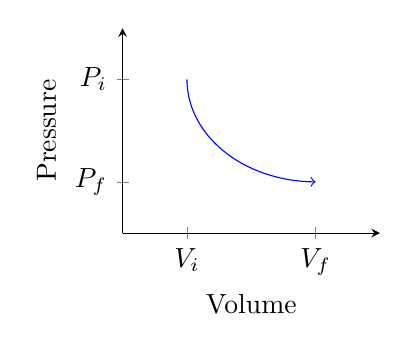
\begin{tikzpicture}
\begin{axis}[
    axis lines=left,
    width=.4\linewidth,
    xmin = 0, xmax = 4,
    ymin = 0, ymax = 4,
    xtick={1,3},
    xticklabels={$V_i$,$V_f$},
    ytick={1,3},
    yticklabels={$P_f$,$P_i$},
    xlabel={Volume},
    ylabel={Pressure}
  ]
\addplot [blue, ->, domain=0:pi/2,samples=50]({3 - 2*cos(deg(x))},{3 - 2*sin(deg(x))});
\end{axis}
\end{tikzpicture}
\end{center}

Adiabatic work is done between any two equlibrium states and is \textit{independent of path}. One can define a function of state as the total adiabtic work done on a system. Lets define this a the total internal energy of the system.

\[ \dif U = - \dif W\tsb{adiabatic}\]

Note the minus `$-$' sign is due to the fact that the total energy of the system increases when work is done \textbf{on} this system.


\end{document}